\documentclass[10pt,a4paper]{article}

\usepackage[margin=0.72in]{geometry}
\usepackage{booktabs}
\usepackage{tabularx}
\usepackage{array}
\usepackage{xcolor}
\usepackage{tikz}
\usepackage{hyperref}
\usepackage{enumitem}
\usepackage{titlesec}
\usepackage{float}
\usepackage{caption}
\usepackage{graphicx}
\graphicspath{{../report_assets/}}

\hypersetup{colorlinks=true, linkcolor=black, urlcolor=blue}
\setlength{\parindent}{0pt}
\setlength{\parskip}{4pt}
\setlist[itemize]{leftmargin=*, topsep=2pt, itemsep=1pt}
\setlist[enumerate]{leftmargin=*, topsep=2pt, itemsep=1pt}
\titleformat{\section}{\large\bfseries}{\thesection}{0.6em}{}
\titleformat{\subsection}{\normalsize\bfseries}{\thesubsection}{0.6em}{}

\begin{document}

\begin{center}
{\Large \textbf{CityFleet Taxi Demand, Revenue \& Fare Quality Control Tower}}\\
\vspace{2pt}
Engineering of Data Analysis --- Assignment 2: Data Pipeline on Databricks \\[5pt]
Noah Kreyenkamp \\[2pt]
Xaver Baeppler \\[4pt]
\end{center}

\section{Business Context and Pipeline Design}

CityFleet is a hypothetical New York taxi fleet operator. Its daily operational problem is that passenger demand changes strongly by hour and location, while management also needs evidence for weekly fleet planning and fare-quality review. The project therefore prototypes a lakehouse pipeline that turns raw taxi trip files into dashboard-ready and self-service analytical tables.

\begin{table}[H]
\centering
\small
\begin{tabularx}{\linewidth}{>{\bfseries}p{0.23\linewidth} X p{0.18\linewidth}}
\toprule
Consumer & Decision supported & Cadence \\
\midrule
Dispatch / operations & Identify pickup hotspots and reposition idle vehicles toward high-demand grid cells. & Hourly \\
Fleet planning & Track trips, revenue, active vehicles, active drivers, payment mix, and coverage patterns. & Weekly \\
Finance / audit & Review suspicious fares, invalid GPS records, zero-distance paid trips, and extreme tips. & Daily / weekly \\
Business analysts & Ask natural-language questions over curated tables using Databricks Genie. & Ad hoc \\
\bottomrule
\end{tabularx}
\end{table}

\begin{figure}[H]
\centering
\resizebox{0.96\linewidth}{!}{%
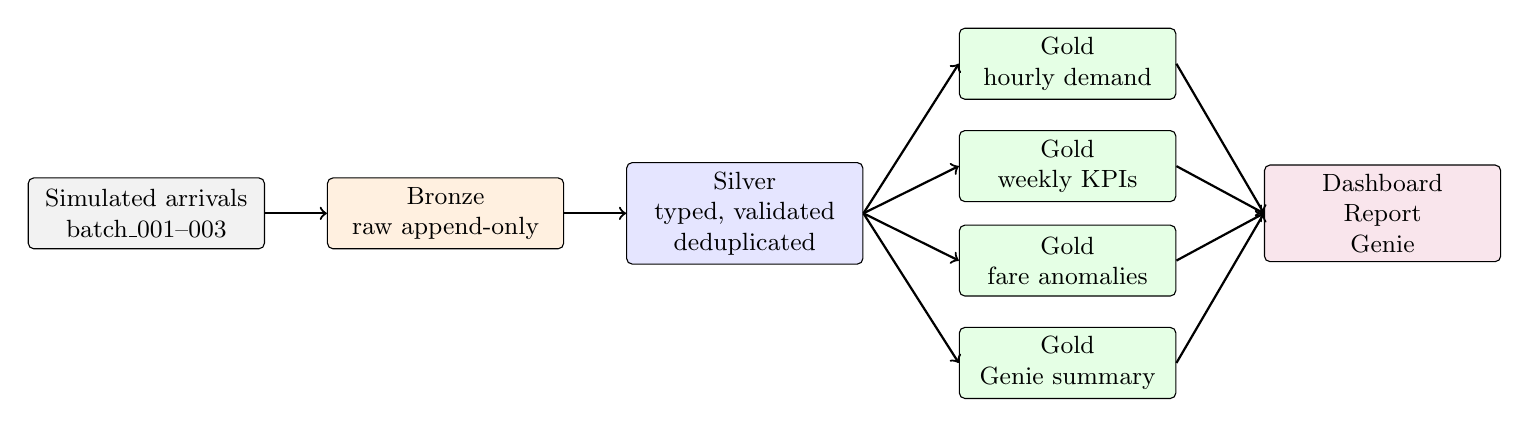
\begin{tikzpicture}[
  box/.style={draw, rounded corners=2pt, align=center, minimum width=3.0cm, minimum height=0.9cm, font=\small},
  goldbox/.style={box, fill=green!10, minimum width=2.75cm},
  arrow/.style={->, thick}
]
\node[box, fill=gray!10] (src) at (0,0) {Simulated arrivals\\batch\_001--003};
\node[box, fill=orange!12] (bronze) at (3.8,0) {Bronze\\raw append-only};
\node[box, fill=blue!10] (silver) at (7.6,0) {Silver\\typed, validated\\deduplicated};
\node[goldbox] (g1) at (11.7,1.9) {Gold\\hourly demand};
\node[goldbox] (g2) at (11.7,0.6) {Gold\\weekly KPIs};
\node[goldbox] (g3) at (11.7,-0.6) {Gold\\fare anomalies};
\node[goldbox] (g4) at (11.7,-1.9) {Gold\\Genie summary};
\node[box, fill=purple!10] (out) at (15.7,0) {Dashboard\\Report\\Genie};
\draw[arrow] (src) -- (bronze);
\draw[arrow] (bronze) -- (silver);
\draw[arrow] (silver.east) -- (g1.west);
\draw[arrow] (silver.east) -- (g2.west);
\draw[arrow] (silver.east) -- (g3.west);
\draw[arrow] (silver.east) -- (g4.west);
\draw[arrow] (g1.east) -- (out.west);
\draw[arrow] (g2.east) -- (out.west);
\draw[arrow] (g3.east) -- (out.west);
\draw[arrow] (g4.east) -- (out.west);
\end{tikzpicture}%
}
\caption{Medallion architecture used in the Databricks prototype.}
\end{figure}

\section{Data Source and Incremental Arrival}

The source is the instructor-provided NYC taxi trip dataset, stored as compressed CSV without a header. The selected sample contains 1,999,999 trips between 2013-01-01 and 2013-01-20. Fields include vehicle id, driver id, pickup/dropoff timestamps, trip duration, distance, pickup/dropoff GPS coordinates, payment type, fare, tip, tolls, and total amount.

Because the source file is static, arrival is simulated by splitting it into time-ordered compressed files. This follows the Lecture 8 pattern: upload a new folder/file, append Bronze, merge Silver, and recompute Gold.

\begin{table}[H]
\centering
\small
\begin{tabular}{llrl}
\toprule
Batch & Date range & Rows & Role \\
\midrule
batch\_001 & 2013-01-01 to 2013-01-04 & 864,187 & Initial load \\
batch\_002 & 2013-01-05 to 2013-01-14 & 599,783 & Refresh iteration 1 \\
batch\_003 & 2013-01-15 to 2013-01-20 & 536,029 & Refresh iteration 2 \\
\bottomrule
\end{tabular}
\end{table}

\section{Medallion Implementation}

\textbf{Bronze.} Table \texttt{bronze\_taxi\_raw} stores the 17 source fields as strings and adds \texttt{source\_file}, \texttt{ingestion\_batch\_id}, \texttt{ingestion\_timestamp}, and \texttt{raw\_row\_hash}. The layer is append-only and preserves source fidelity.

\textbf{Silver.} Table \texttt{silver\_taxi\_trips} casts timestamps and numeric columns, creates a deterministic \texttt{trip\_id}, computes pickup/dropoff grid cells, and stores quality flags. Validation rules check NYC-area coordinates, non-null ordered timestamps, positive duration and distance, non-negative fare/tip, and positive total amount. New batches are merged by \texttt{trip\_id}, making Silver the deduplicated source of truth.

\textbf{Refresh schedule.} In the prototype, the pipeline is triggered manually: one run of notebook \texttt{02\_incremental\_refresh} per simulated arrival. The intended production schedule is: Bronze and Silver refresh on each file arrival (event-driven or every 15~minutes for the operational path); \texttt{gold\_hourly\_demand\_by\_cell} and \texttt{gold\_genie\_taxi\_summary} refresh every 15~minutes; \texttt{gold\_weekly\_fleet\_kpis} refreshes nightly; \texttt{gold\_fare\_anomaly\_review} refreshes daily.

\textbf{Gold.} Four curated tables serve distinct consumers:

\begin{table}[H]
\centering
\small
\begin{tabularx}{\linewidth}{>{\ttfamily}p{0.33\linewidth} X}
\toprule
\textrm{Gold table} & Purpose \\
\midrule
gold\_hourly\_demand\_by\_cell & Operational dashboard with trip counts, active vehicles/drivers, revenue, payment mix, and demand score by pickup cell and hour. \\
gold\_weekly\_fleet\_kpis & Strategic reporting table with weekly trips, revenue, active vehicles, active drivers, card/cash share, trips per vehicle, and revenue per vehicle. \\
gold\_fare\_anomaly\_review & Audit queue for high fares, zero-distance paid trips, high tip ratios, nonpositive durations, and invalid coordinates. \\
gold\_genie\_taxi\_summary & Business-readable hourly table with clearer column names for Genie self-service questions. \\
\bottomrule
\end{tabularx}
\end{table}

\begin{figure}[H]
\centering
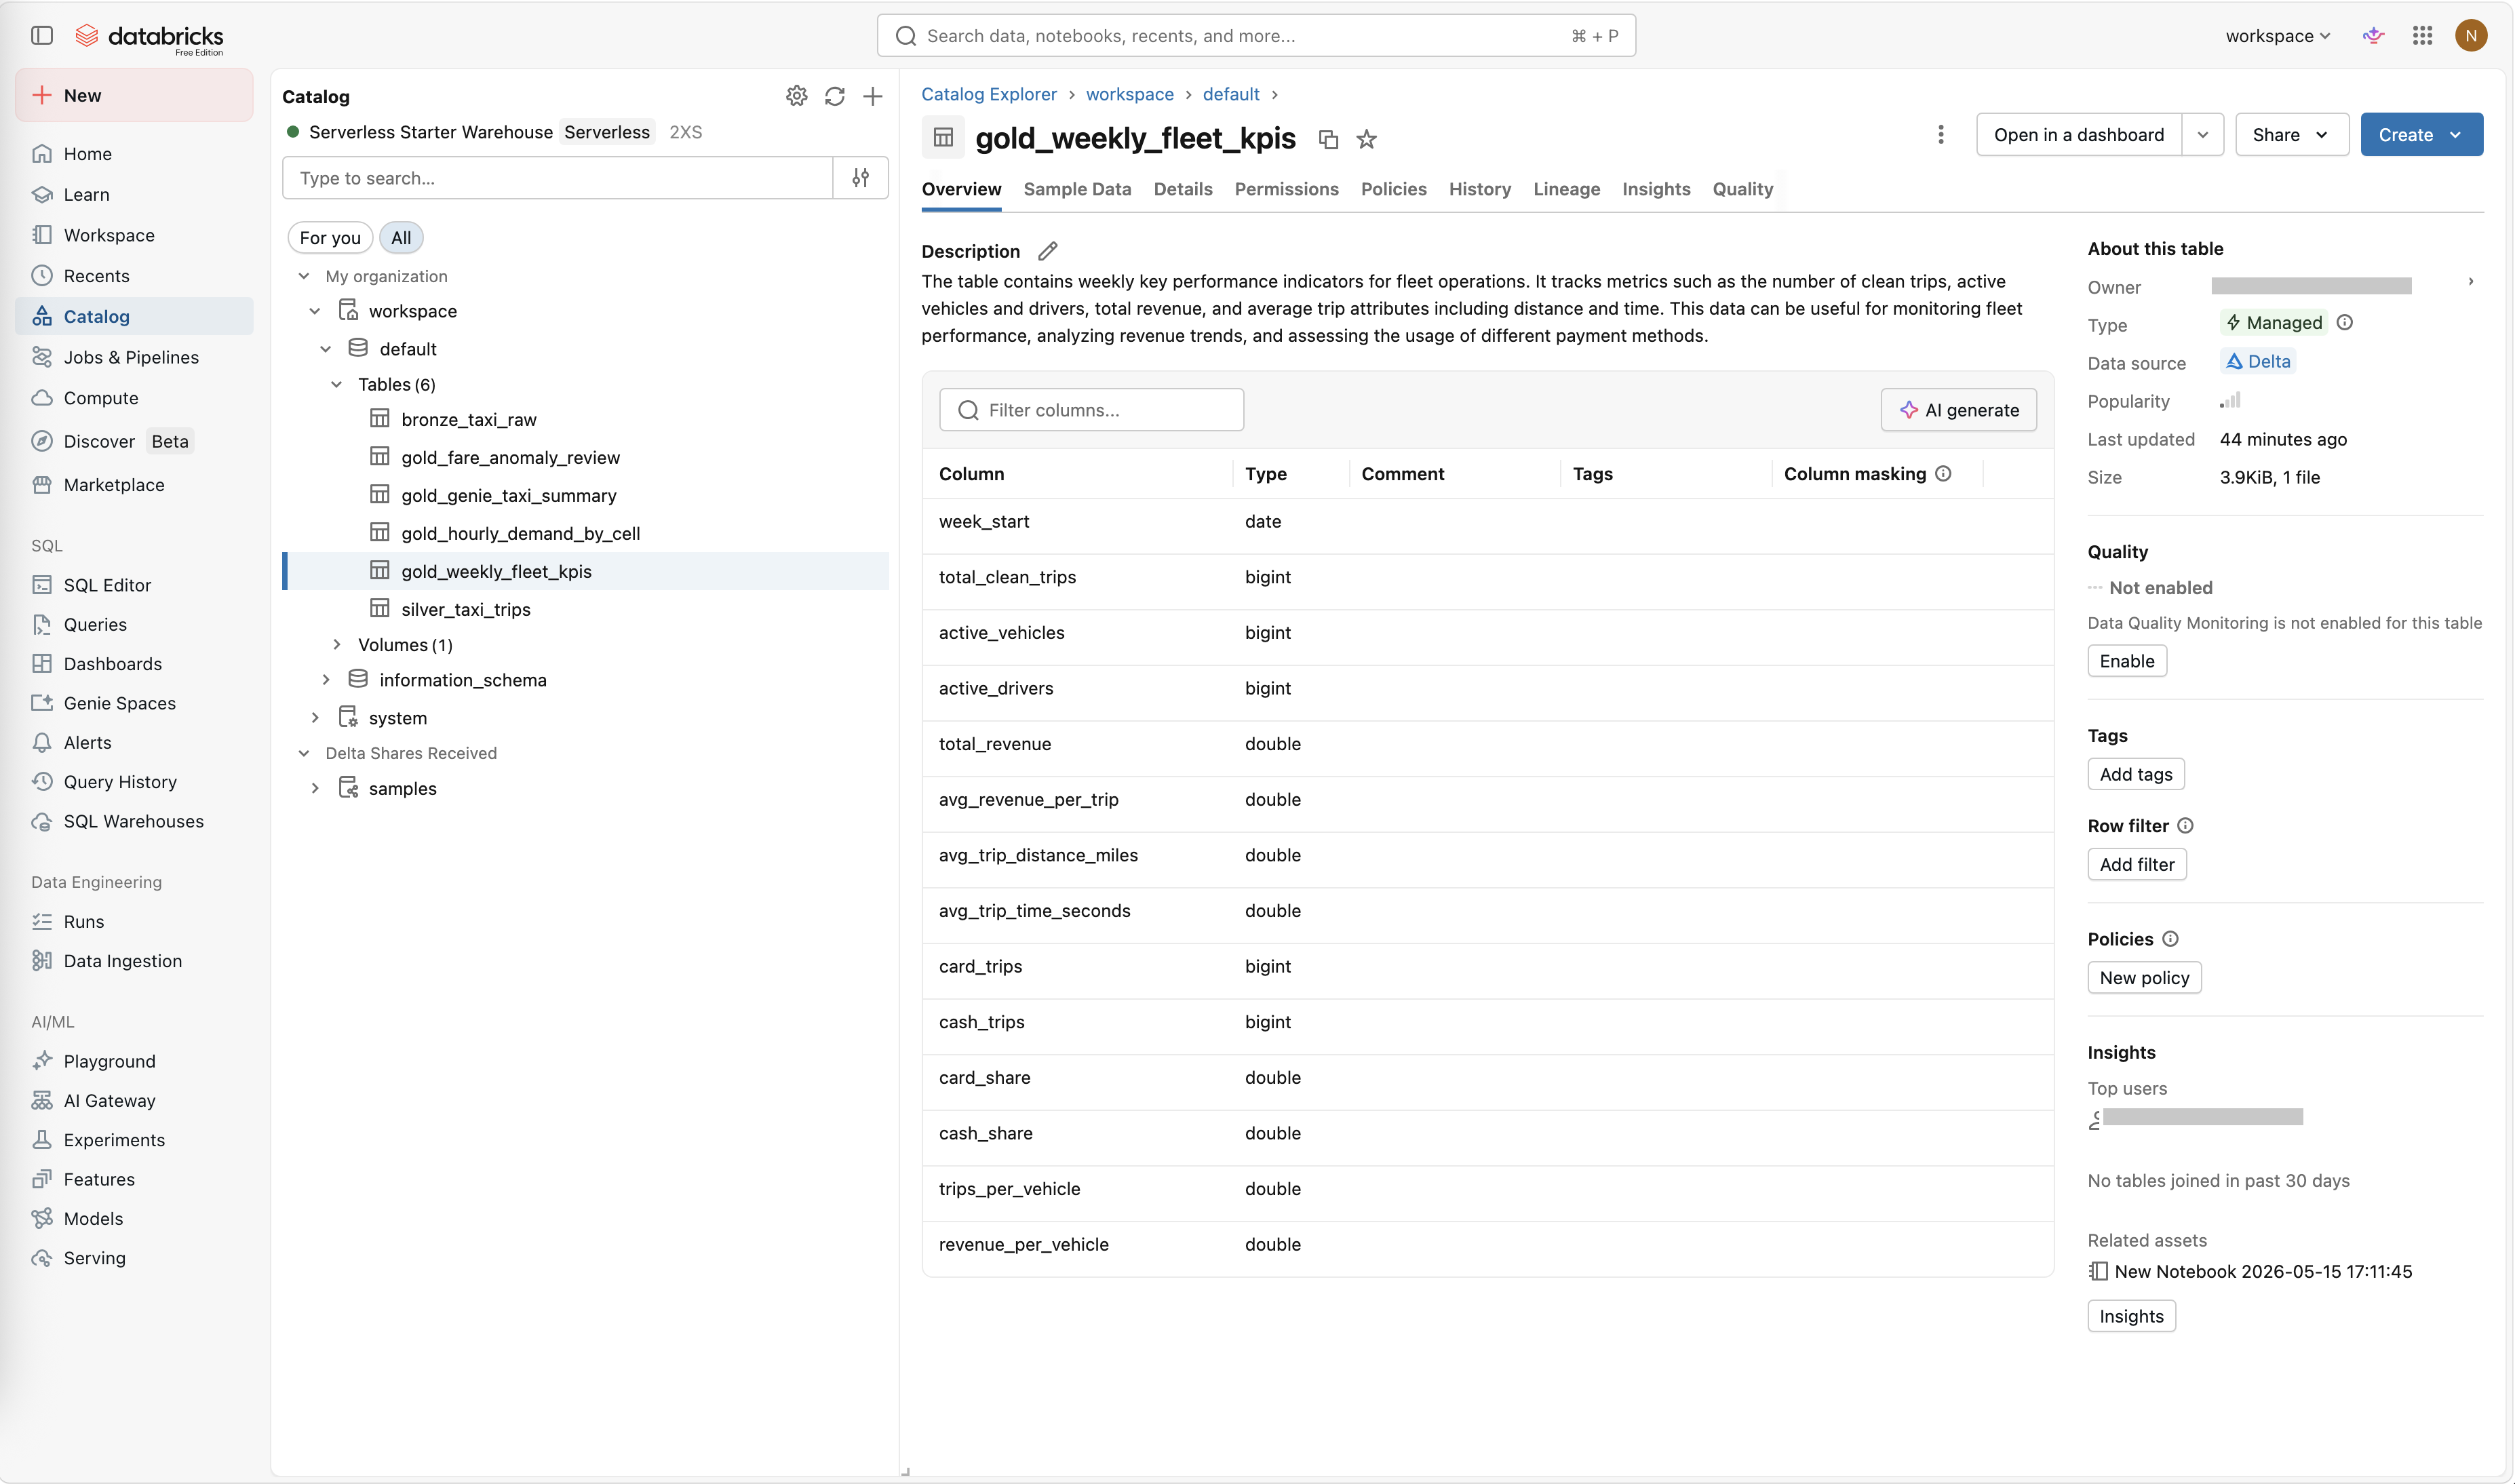
\includegraphics[width=0.92\linewidth]{databricks_gold_kpi_table.png}
\caption{Databricks Unity Catalog view of \texttt{gold\_weekly\_fleet\_kpis} showing the implemented column schema and table metadata.}
\end{figure}

\section{Outputs and Business Actions}

The implemented end-to-end consumer is a Databricks Genie space connected to the curated Gold layer \\ (\texttt{gold\_genie\_taxi\_summary}, \texttt{gold\_weekly\_fleet\_kpis}, and \texttt{gold\_fare\_anomaly\_review}). The Gold tables are also dashboard-ready; notebook \texttt{03\_dashboard\_and\_genie\_queries} contains four parameterised SQL queries that map to suggested tiles: latest-hour demand hotspots, hourly demand and revenue trend, weekly fleet KPI table, and fare anomaly review queue. These outputs map directly to actions: operations can guide drivers toward high-demand cells; planners can adjust weekly coverage and incentives; finance can investigate suspicious fare records; analysts can use Genie without querying raw data.

The validation notebook processed all three simulated arrivals and produced these cumulative counts: after \texttt{batch\_001}, Bronze and Silver contained 864,187 trips and 845,368 clean trips; after \texttt{batch\_002}, Bronze and Silver contained 1,463,970 trips and 1,431,432 clean trips; after \texttt{batch\_003}, Bronze and Silver contained 1,999,999 trips and 1,955,237 clean trips. The final Gold tables contained 314,394 hourly demand rows and 45,382 fare anomaly review rows.

\begin{figure}[H]
\centering
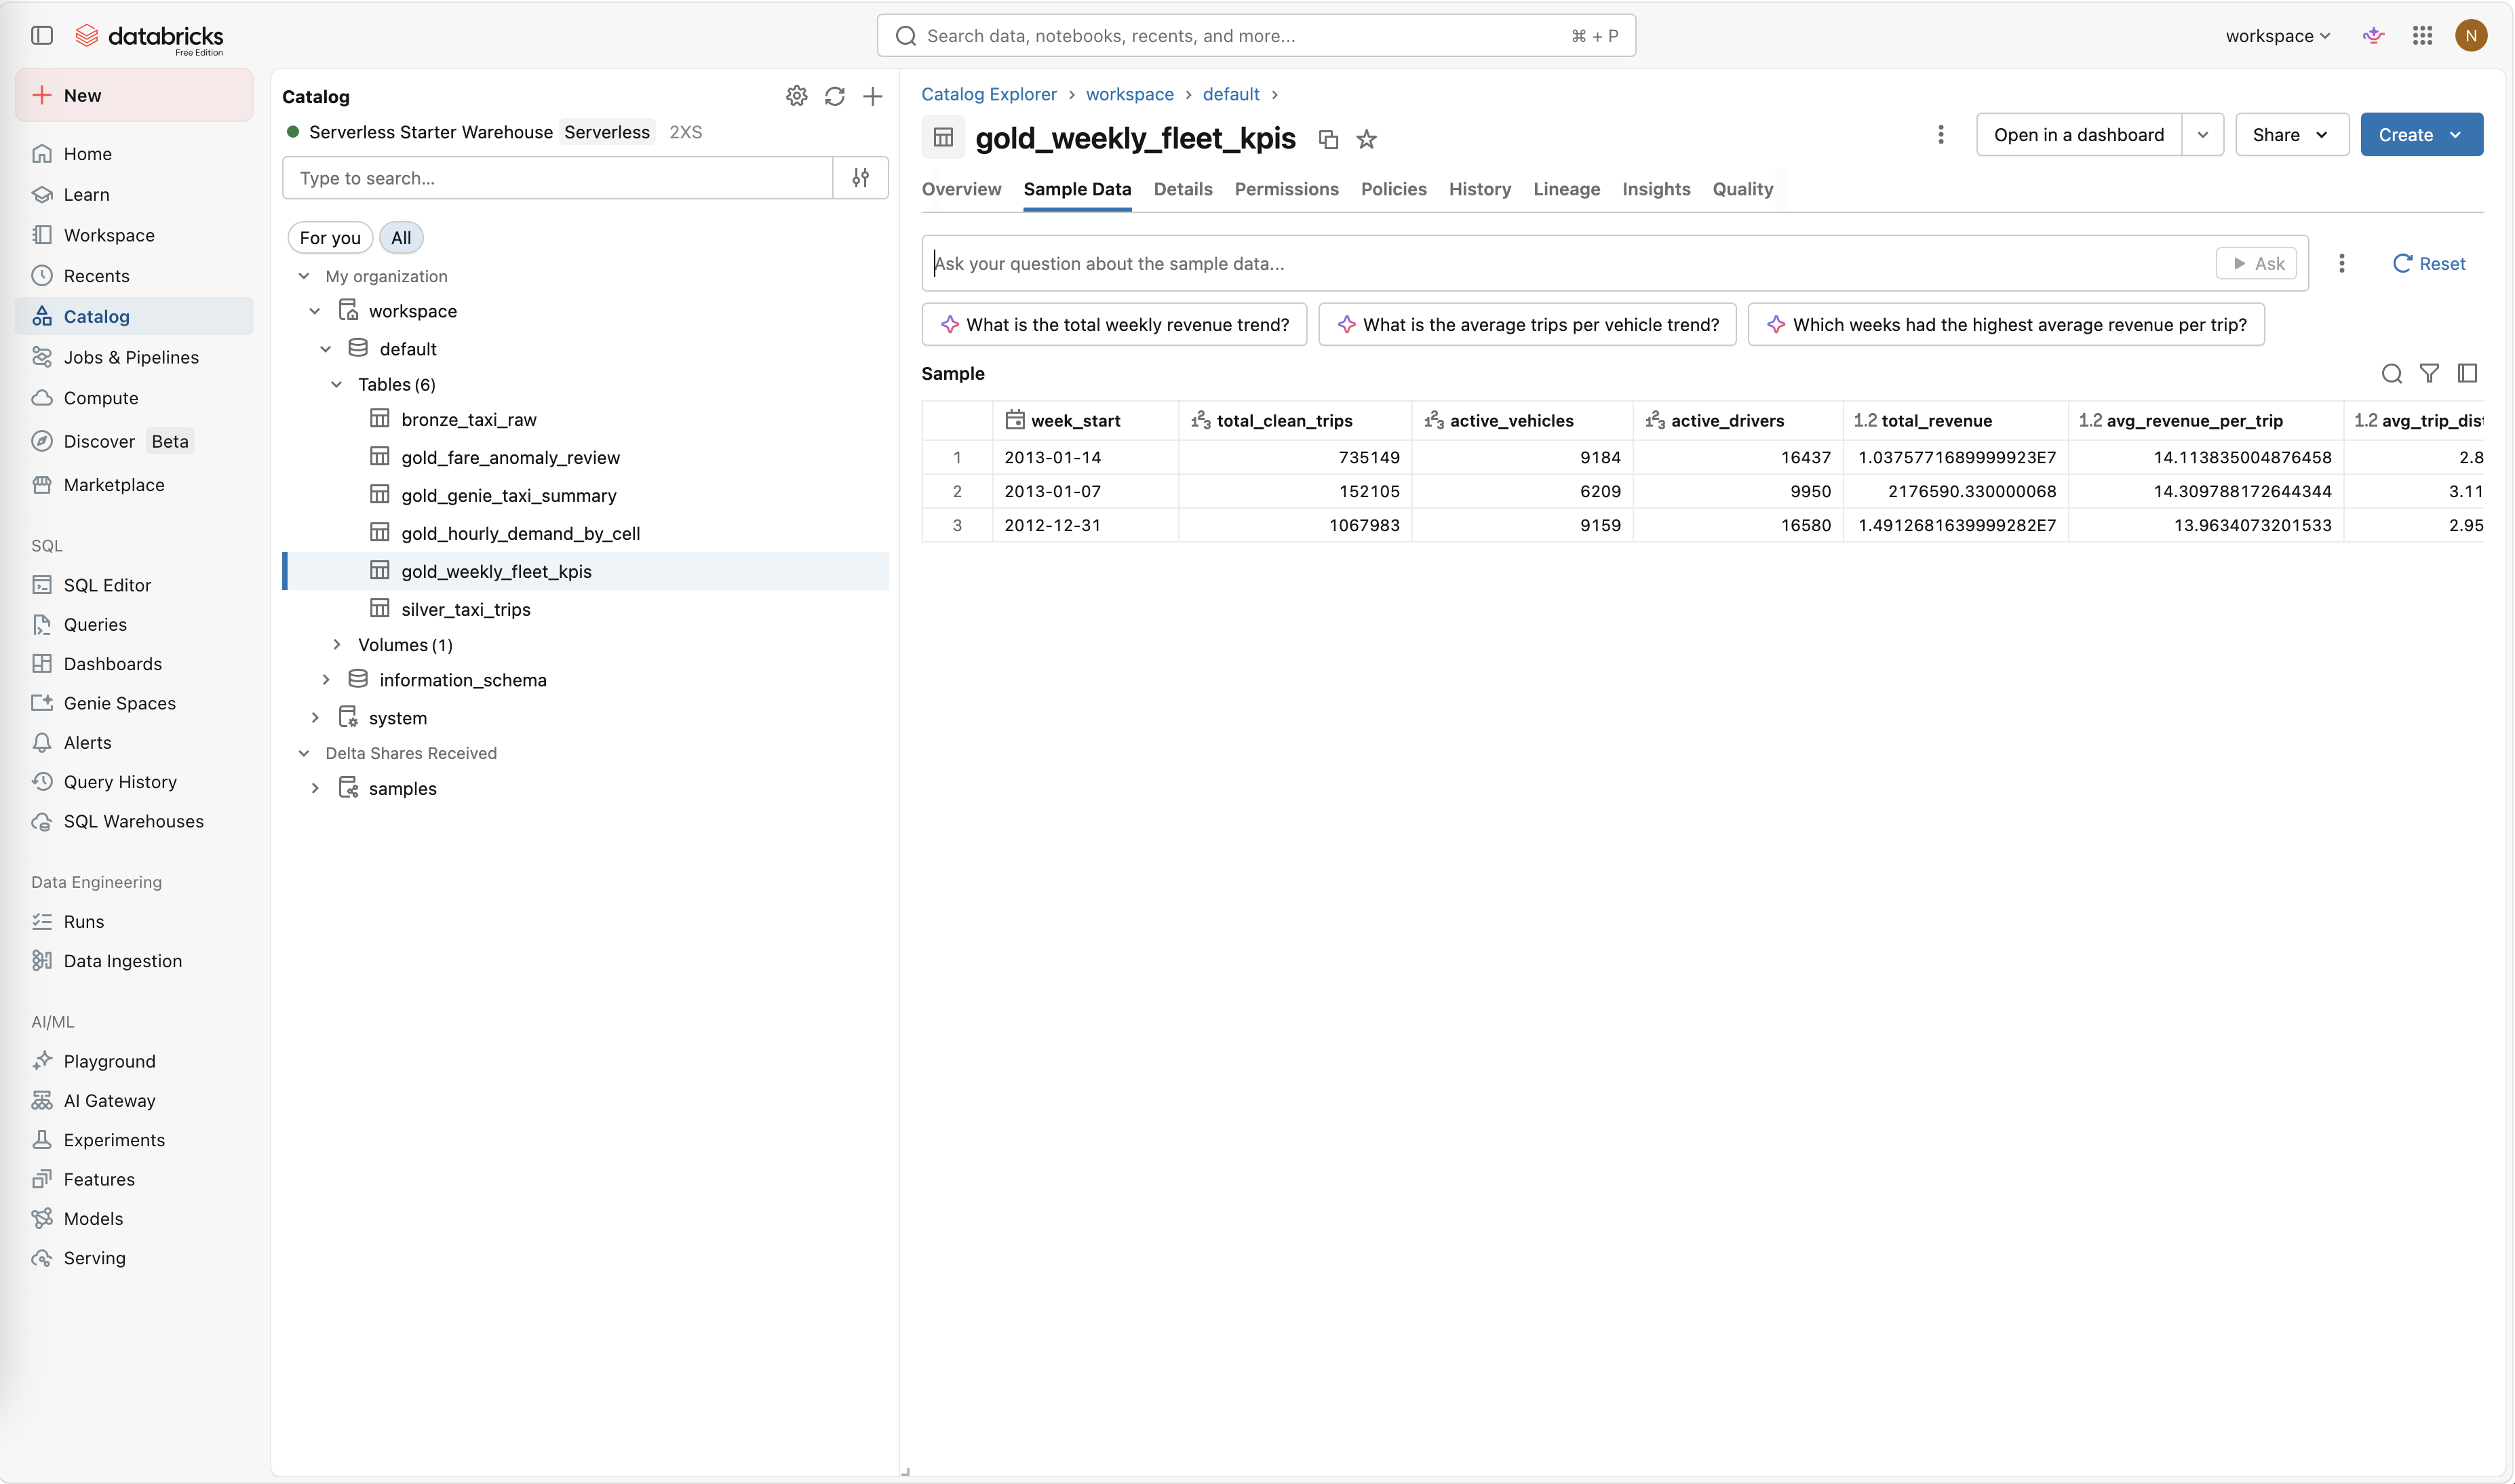
\includegraphics[width=0.92\linewidth]{databricks_gold_kpi_sample.png}
\caption{Databricks Catalog sample for the weekly strategic Gold KPI table.}
\end{figure}

\begin{figure}[H]
\centering
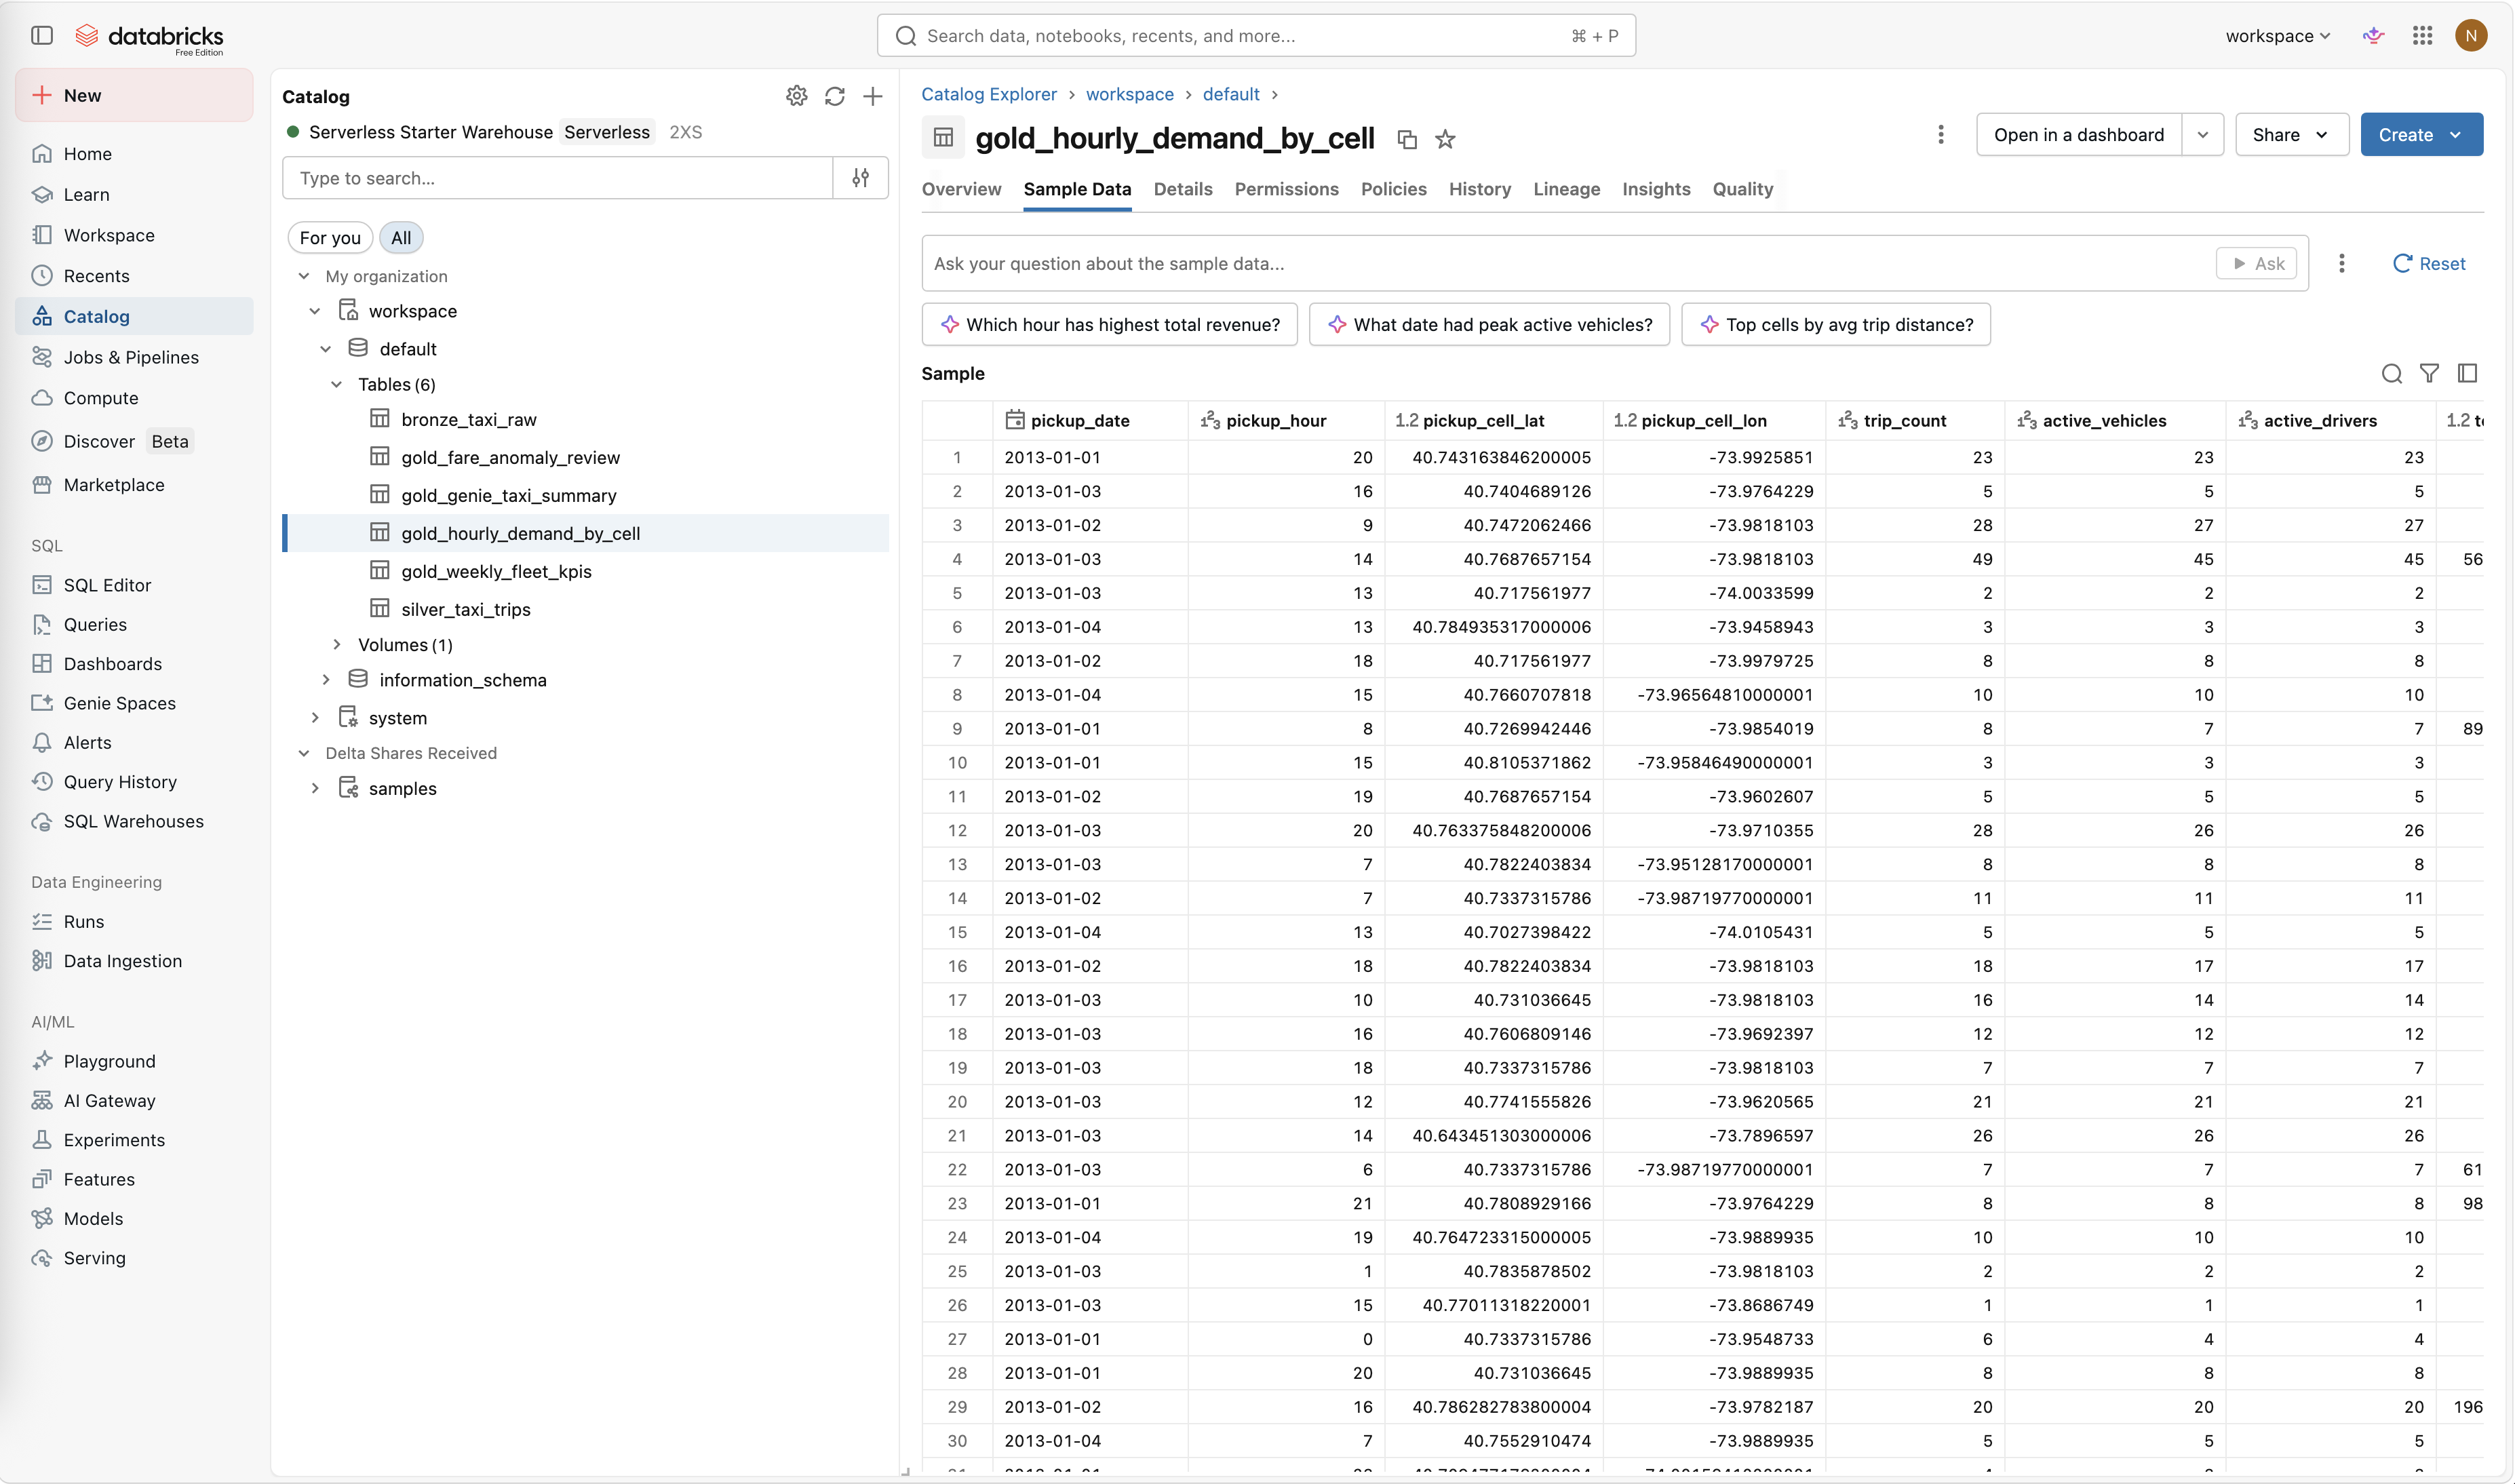
\includegraphics[width=0.92\linewidth]{databricks_gold_hourly_sample.png}
\caption{Databricks Catalog sample for the operational hourly demand Gold table.}
\end{figure}

\section{Genie Experience}

Genie was tested against Gold tables rather than Bronze/Silver because Genie performs best when table grain and column names are business-readable. The main table for Genie is \texttt{gold\_genie\_taxi\_summary}, supported by \texttt{gold\_weekly\_fleet\_kpis} and \texttt{gold\_fare\_anomaly\_review}.

\textbf{Questions that worked.} ``Which service date and hour had the highest number of taxi trips? Show the top 5 with trip counts.'' worked well because it matched the Gold table grain exactly. Other successful questions:

\begin{itemize}
\item Which pickup areas had the highest demand score in the latest available hour?
\item How did total revenue and active vehicles change by week?
\item What are the most common fare anomaly reasons?
\item Which hours have the highest card payment share?
\end{itemize}

\textbf{Questions that failed or required schema changes.} Questions using the word ``hotspot'' (e.g.\ ``Show me the current demand hotspots'') initially returned no results or a generic table dump because Genie could not map ``hotspot'' to any column. The fix was to add the column \texttt{demand\_score} with a table comment explaining that higher values indicate busier pickup areas, and to rename coordinate columns to \texttt{pickup\_area\_latitude} and \texttt{pickup\_area\_longitude} so Genie could infer geographic intent. After these changes, geographic demand questions answered correctly. Similarly, questions referencing ``revenue per driver'' failed until \texttt{active\_drivers} was included in the Genie table alongside revenue columns, giving Genie enough context to compute the ratio without hallucinating column names.

\begin{figure}[H]
\centering
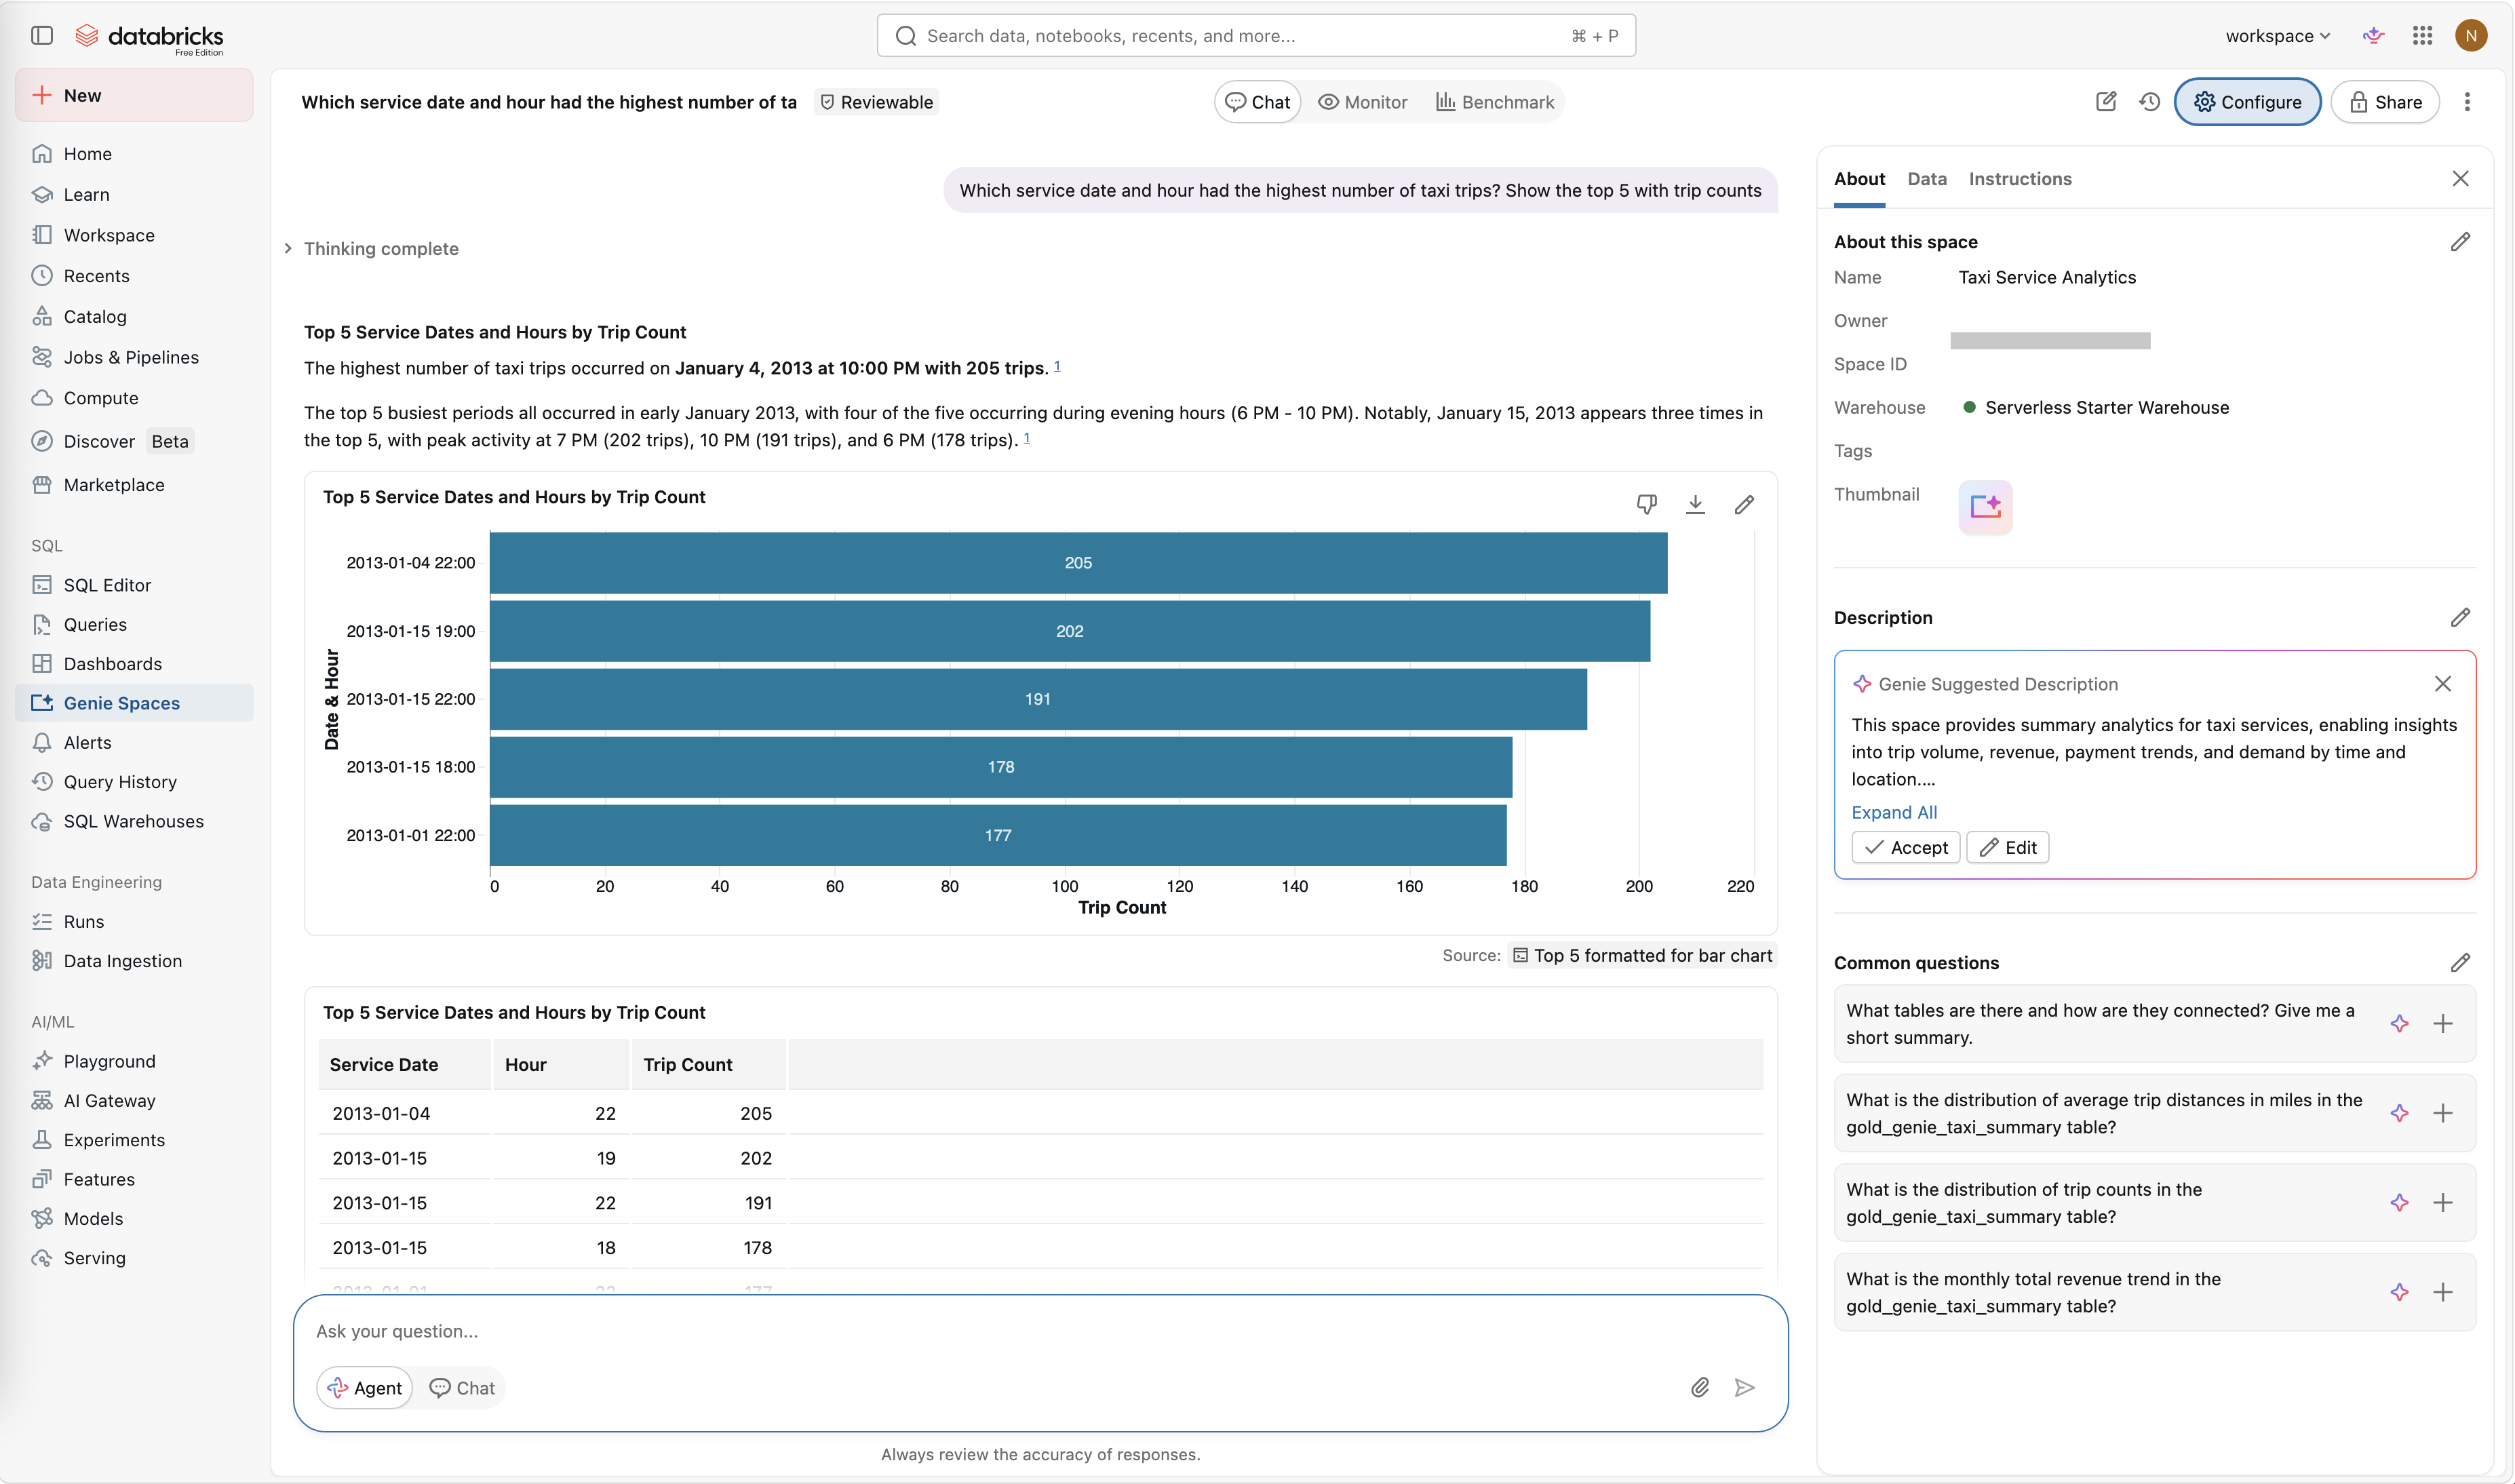
\includegraphics[width=0.92\linewidth]{genie_answer.png}
\caption{Databricks Genie successfully answering an ad hoc business question from a curated Gold table.}
\end{figure}

\section{Production Discussion}

The prototype runs on Databricks Free Edition using manual file upload and simulated arrivals. In production, raw trip events would land automatically. Periodic files could be ingested with Auto Loader from S3, Azure Blob, or GCS; continuous dispatch events could arrive through Kafka or Event Hubs and be processed with Structured Streaming. Compute would move from quota-limited serverless execution to scheduled jobs or multi-node clusters. Storage would move from workspace volumes to governed cloud object storage. Unity Catalog would manage access control, lineage, and table permissions. Monitoring would track missing files, job failures, freshness, data-quality failure rates, and anomaly volumes.

At full scale, Bronze would retain raw history cheaply, Silver would be partitioned by pickup date, and Gold tables would be refreshed incrementally rather than fully recomputed. The operational table could refresh every 5--15 minutes, while strategic KPIs could refresh nightly or weekly.

\newpage
\section*{AI Tools Usage}

AI tools used:
OpenAI Codex was used in the Codex desktop environment as an AI-assisted development tool. The work was collaborative and agentic, but the main design decisions, validation steps, and final project choices were made by the students. Codex helped us interpret the project requirements, explore and profile the provided datasets, compare suitable dataset options, generate initial batch files, draft Databricks notebook code, and structure parts of the report. We then reviewed, adapted, and tested the generated code and design decisions ourselves.

Development strategy:
Our development followed a design-first and schema-guided approach. We first analysed the assignment rubric and selected a dataset and organisational process that fit the expected requirements. Based on this, we designed the Bronze, Silver, and Gold layers and defined how the data should flow through the pipeline. While AI supported us in drafting much of the Spark/SQL implementation, we adjusted the logic, schemas, and transformations to fit our specific use case. The Gold tables were refined to support both dashboard queries and Genie self-service questions.

Reflection:
AI was most useful for turning the assignment requirements into a concrete implementation plan and for quickly producing a first version of the Spark/SQL notebook code. However, the project still required substantial manual work from our side. We had to understand the dataset, decide on the architecture, validate the outputs in Databricks, debug issues during execution, test the dashboard and Genie results, and select the final screenshots and wording for submission. This meant that we still had to actively test and refine the solution in Databricks ourselves, especially for file uploads, notebook execution, table creation, dashboard behaviour, Genie questions, and final output validation.

\end{document}
